\begin{landscape}
\begin{figure*}[!htbp]
    \centering
    \begin{subfigure}[t]{0.625\textwidth}
        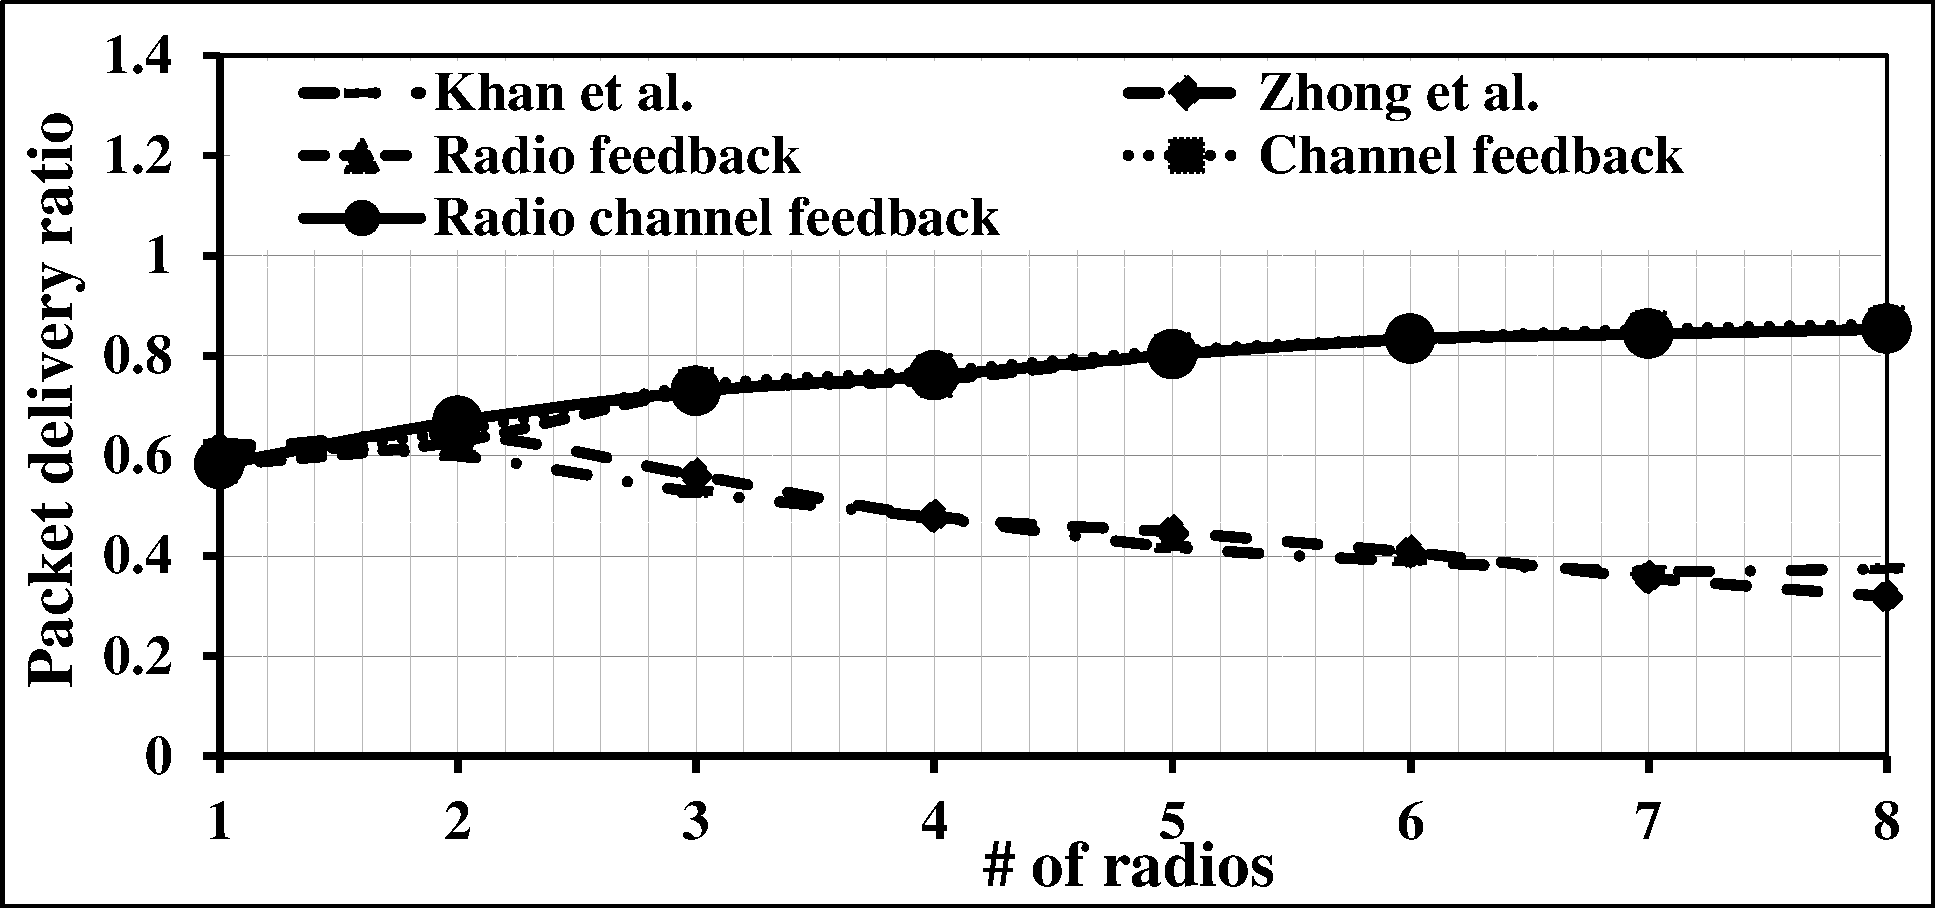
\includegraphics[width=\textwidth]{alltopology/12DeliveryRatio24d1}
        \caption{1Mbps application data rate}
    \end{subfigure}
    ~
    \begin{subfigure}[t]{0.625\textwidth}
        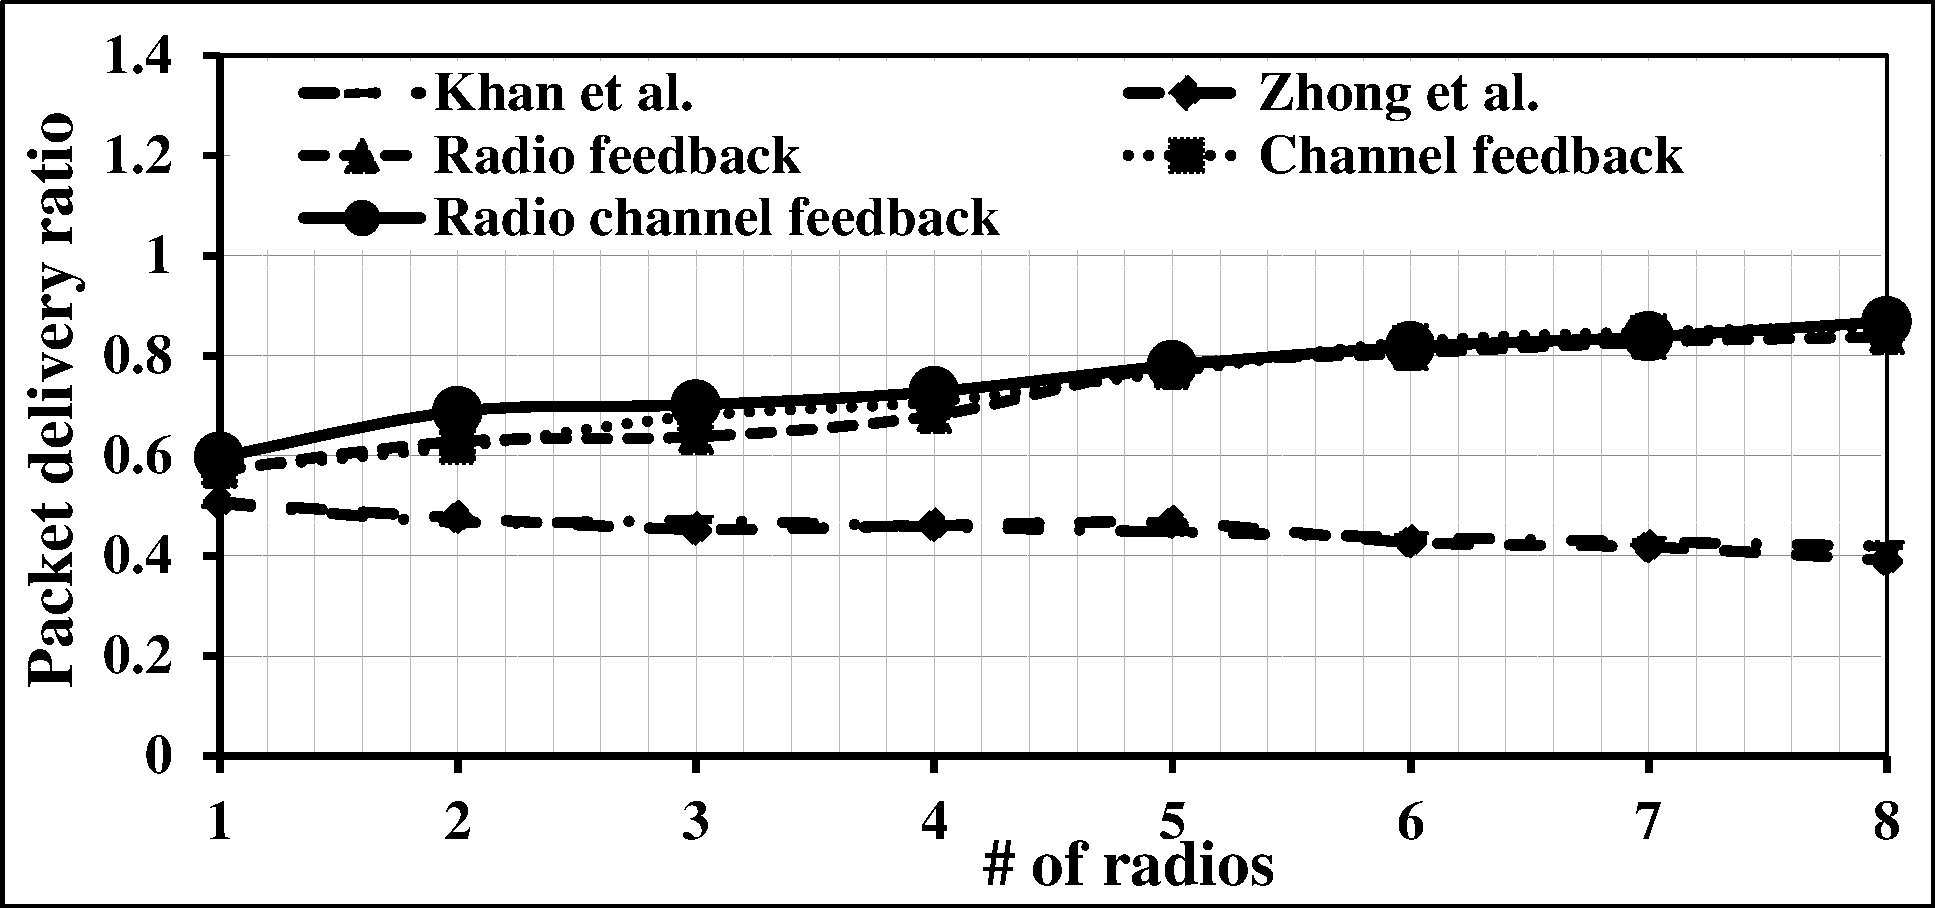
\includegraphics[width=\textwidth]{alltopology/12DeliveryRatio24d2}
        \caption{2Mbps application data rate}
    \end{subfigure}
    ~\\
    \begin{subfigure}[t]{0.625\textwidth}
        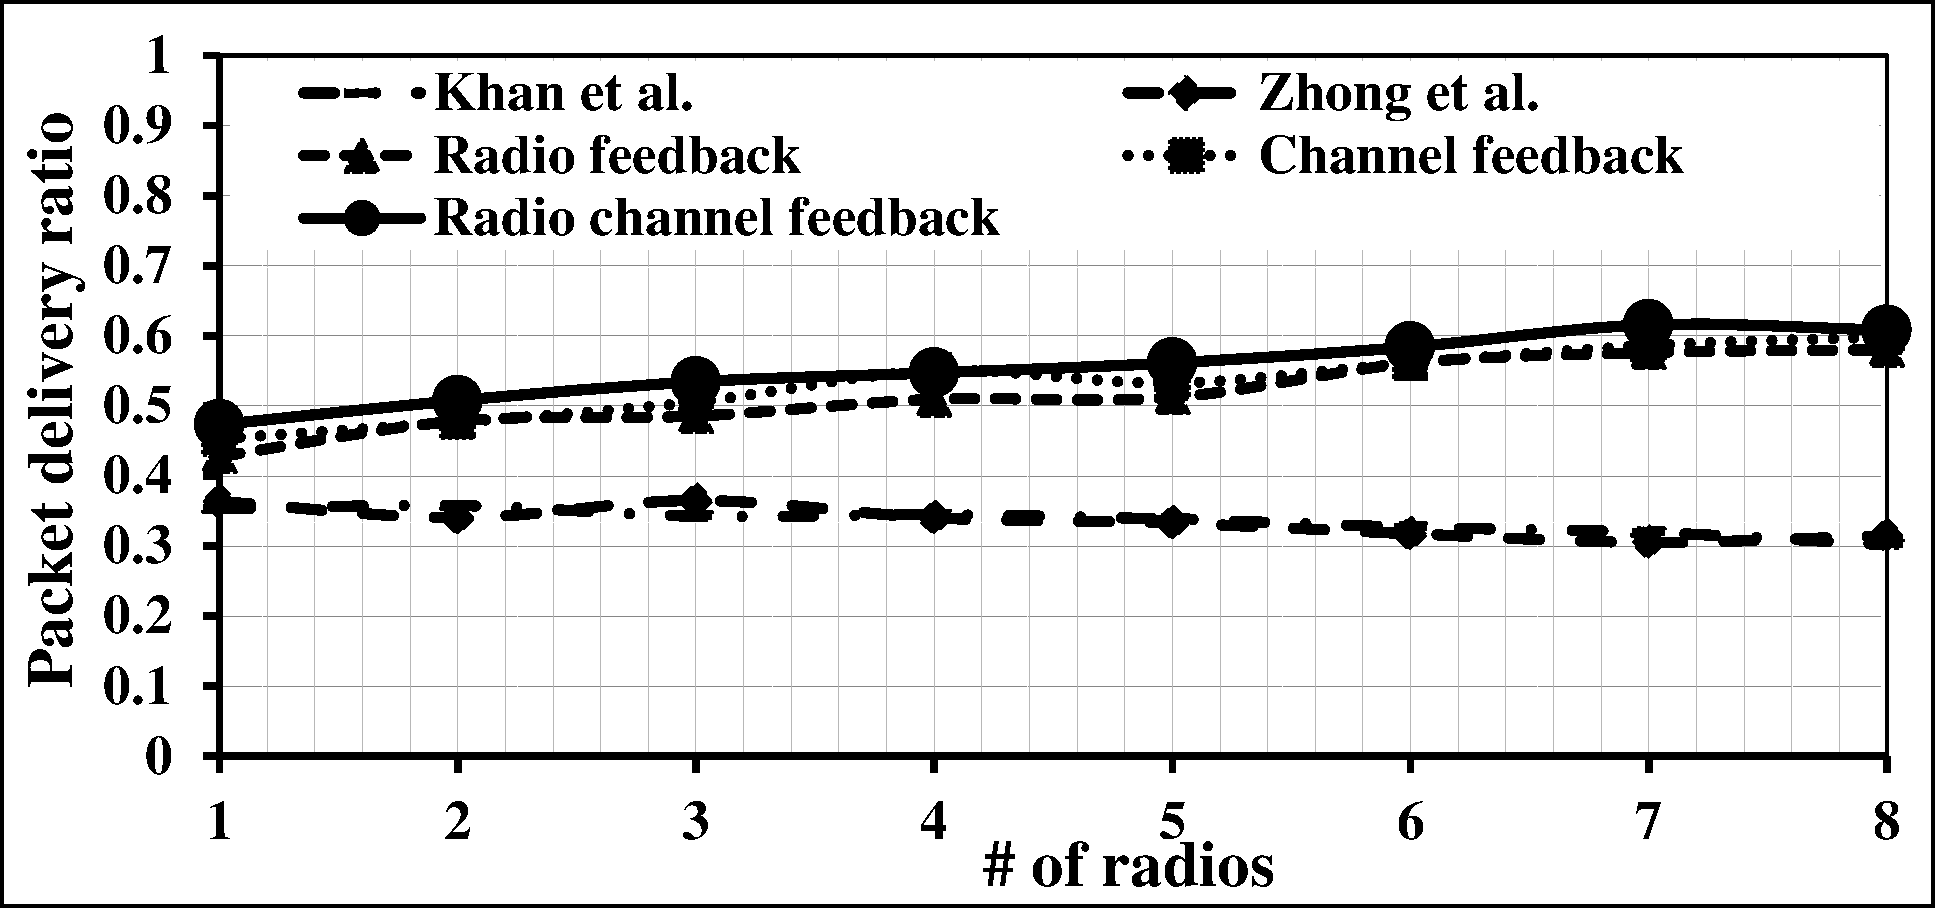
\includegraphics[width=\textwidth]{alltopology/12DeliveryRatio24d4}
        \caption{4Mbps application data rate}
    \end{subfigure}
    ~
    \begin{subfigure}[t]{0.625\textwidth}
        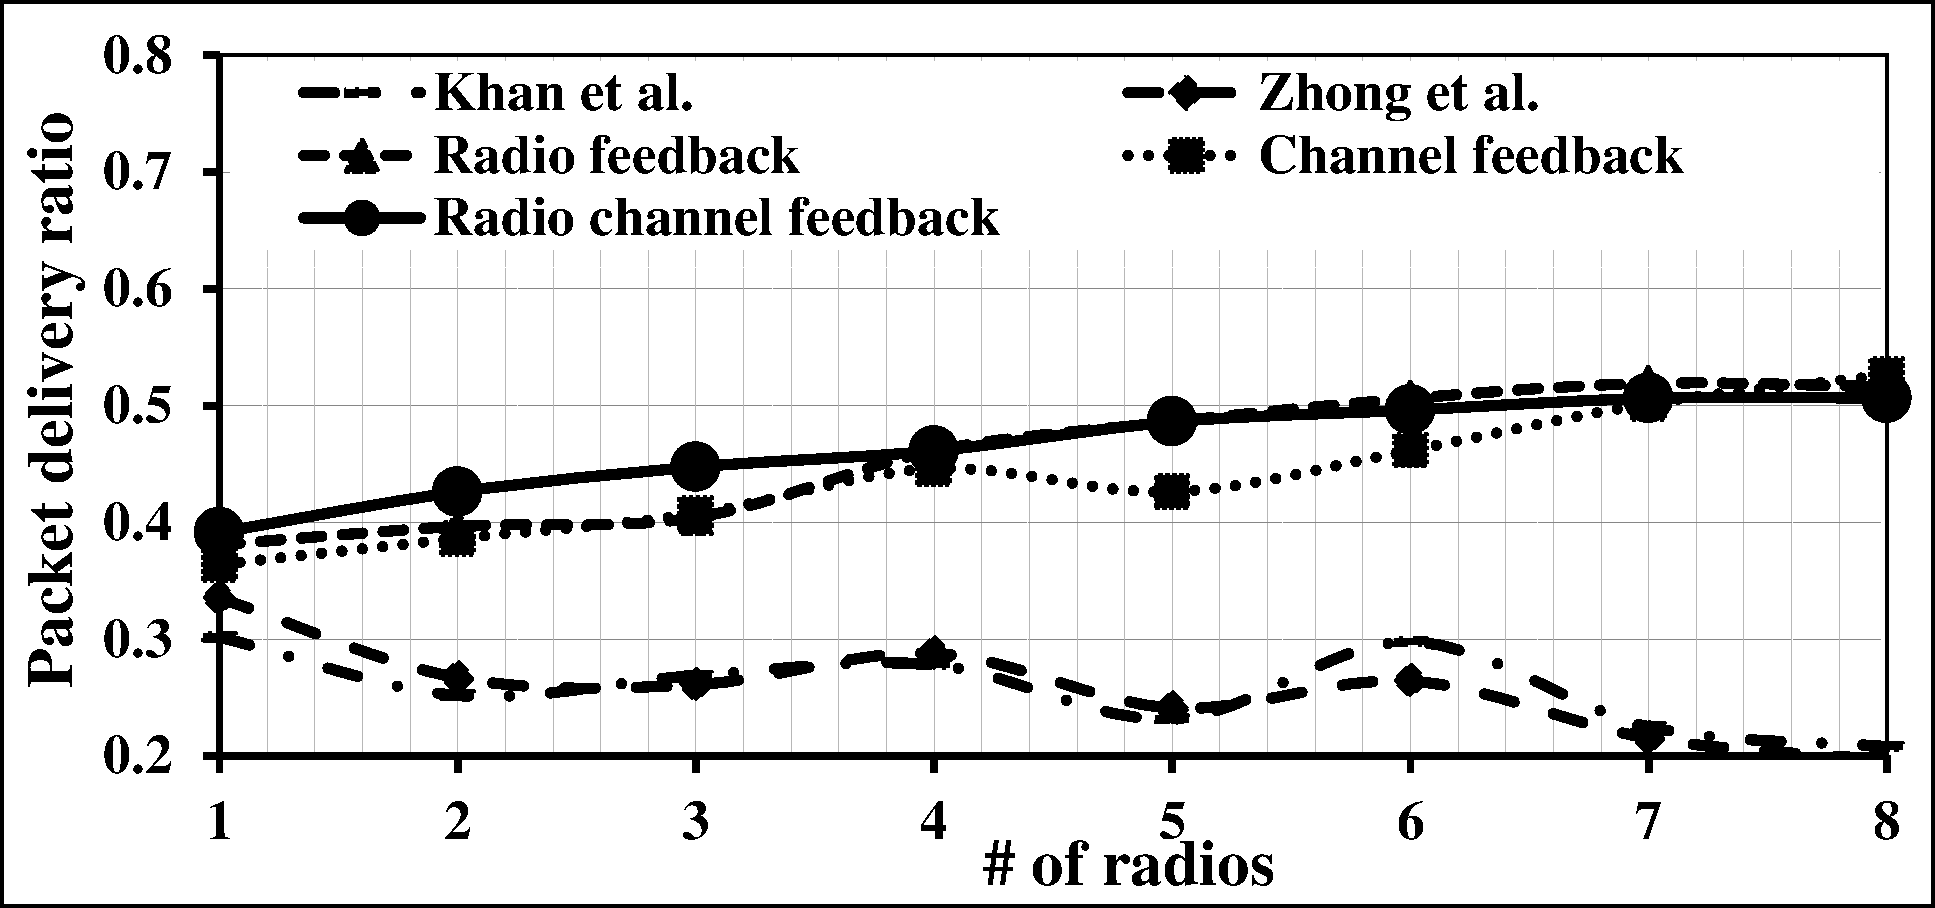
\includegraphics[width=\textwidth]{alltopology/12DeliveryRatio24d8}
        \caption{8Mbps application data rate}
    \end{subfigure}
    ~\\
    \begin{subfigure}[t]{0.625\textwidth}
        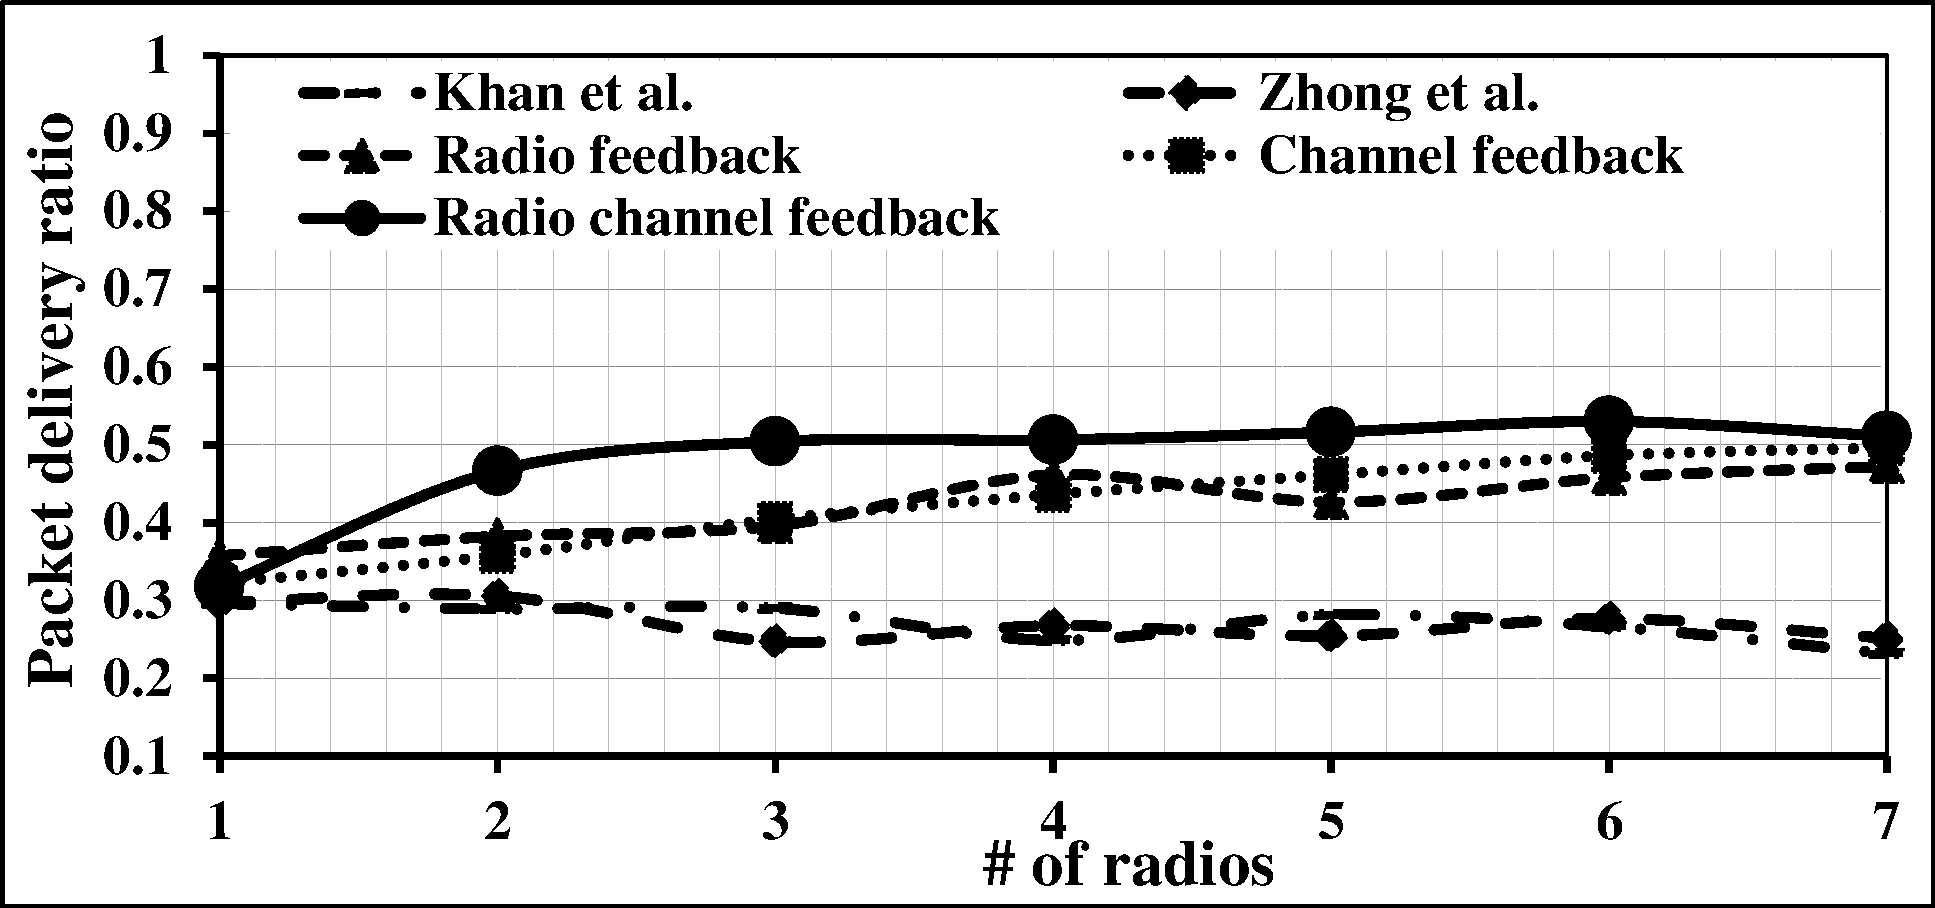
\includegraphics[width=\textwidth]{alltopology/12DeliveryRatio24d16}
        \caption{16Mbps application data rate}
    \end{subfigure}
    ~
    \begin{subfigure}[t]{0.625\textwidth}
        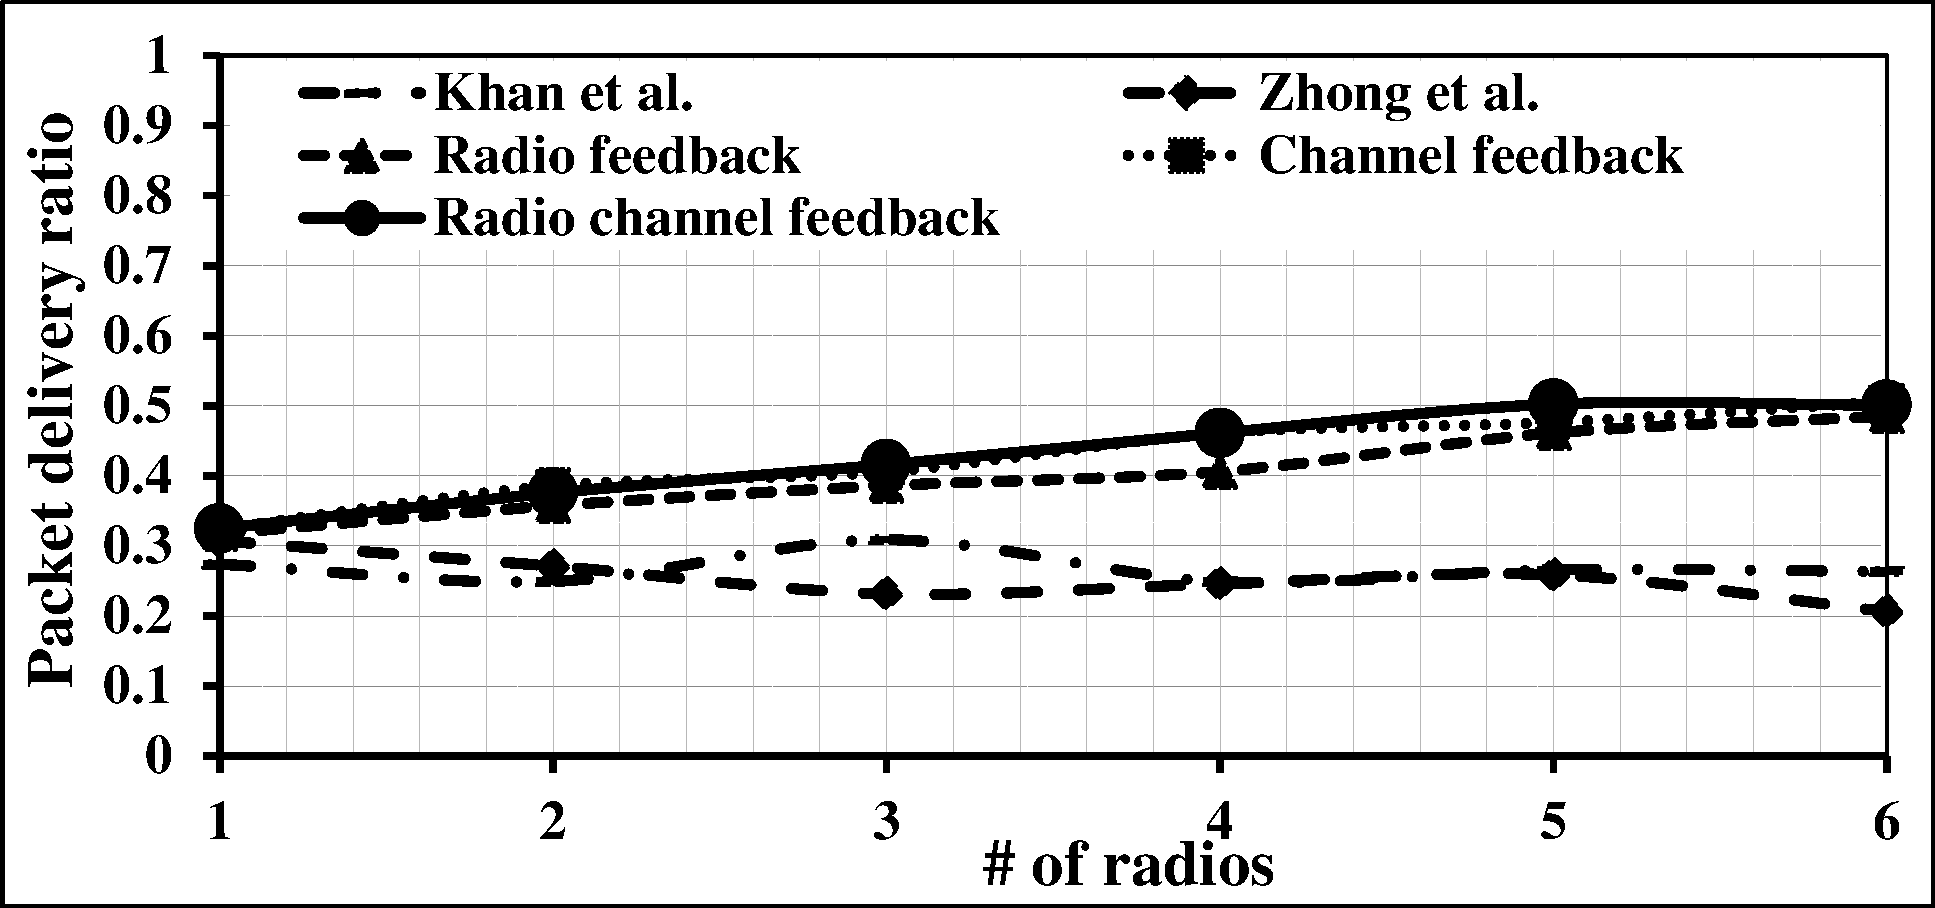
\includegraphics[width=\textwidth]{alltopology/12DeliveryRatio24d32}
        \caption{32Mbps application data rate}
    \end{subfigure}
    \caption{Application layer packet delivery ratio with varying number of radios for various application data rates on a network topology with 12 secondary users}
\end{figure*}
\end{landscape}
